%!TEX root = ../../main.tex
\frame{
	\frametitle{Im Experiment}
	\begin{description}
		\item[Feature Points per Model] 1000
	\end{description}
	\centering
		\textbf{Versuch 1}~~~~~~~~~~~~~\textbf{Versuch 2}~~~~~~~~~~~~~\textbf{Versuch 3}
		\begin{columns}[t]
	 	
    	\begin{column}{4cm}
    	\centering


    	\begin{itemize}
    		\item 6 Modelle aus Stanford 3D Scanning Repository
    		\item Mit jeweils einigen Modellen 45 Szenen erzeugt
    		\item 45 Szenen mit Gaussrauschen versetzt $(\sigma \in {0.1,0.2,0.3})$.
    	\end{itemize} 

     	\end{column}
    	\begin{column}{4cm}
    	\centering
    	\begin{itemize}
    		\item Szenen aus Versuch 1
    		\item Subsampling $f = \frac{1}{8}$
    		
    	\end{itemize} 
    	\end{column}
    	\begin{column}{4cm}
    	\begin{itemize}
    	    			\item 8 Modelle, im Labor erzeugt mit Spacetime-Stereo.
    			\item 15 Szenen, die jeweils zwei der acht Objekte enthalten.	
    		\end{itemize}  
    	
    	\end{column}
    \end{columns}

}


\subsection{Bewertung}
\frame{
	\frametitle{False-Posives?}
	\centering
		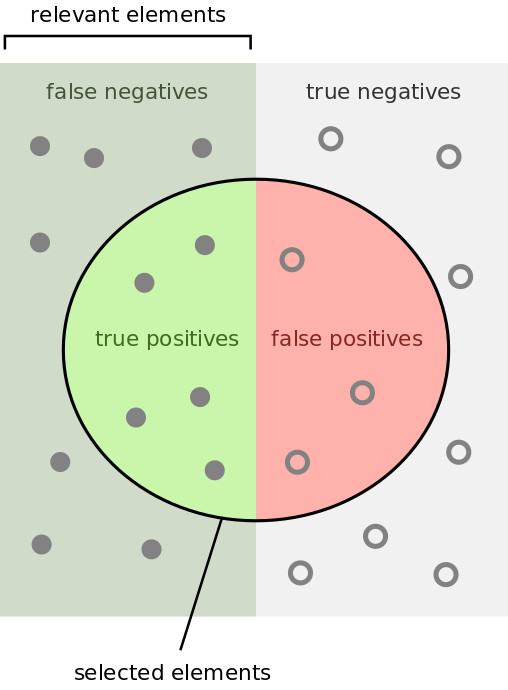
\includegraphics[height=0.8\textheight]{topics/vergleich/pr.jpg}
}

%%Precision recall
\frame{
	\frametitle{Die Maße: Precision und Recall}
	\begin{columns}[c]
    	\begin{column}{5cm}
     		Wie viele der gelieferten Muster sind relevant?
     		$$Precision = \frac{|TP|}{|TP|+|FP|}$$
     		Wie viele der richtigen Muster wurden geliefert? 
     		$$ Recall\frac{|TP|}{|TP|+|FN|}$$
     	\end{column}
    	\begin{column}{5cm}
     		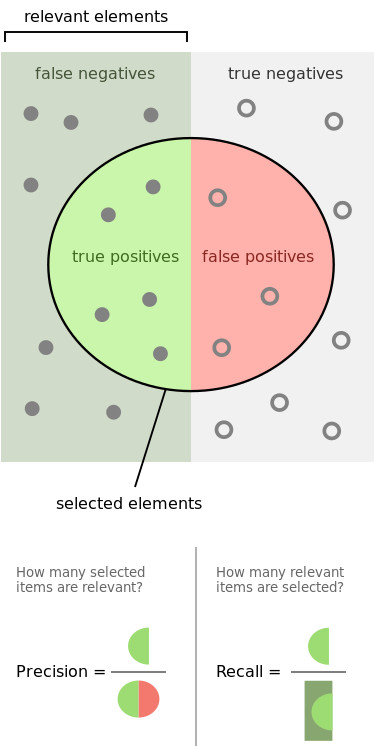
\includegraphics[height=0.8\textheight]{topics/vergleich/pr2.jpg}
    	\end{column}
    \end{columns}
}


\subsection{Ergebnisse}
\frame{
	\frametitle{Ergebnis: Versuch 1}
	\centering
	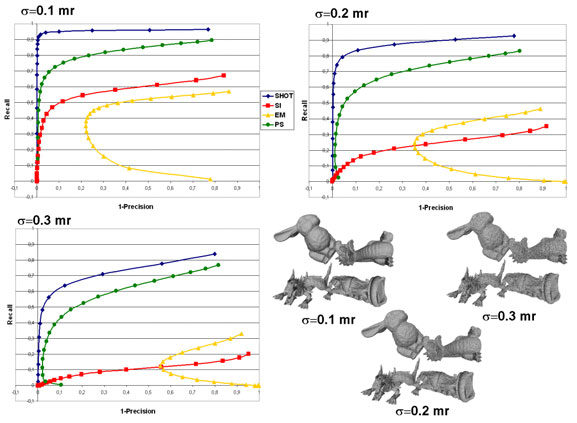
\includegraphics[height=0.8\textheight]{topics/vergleich/v1.png}
}

\frame{
	\frametitle{Ergebnis: Versuch 2}
	\centering
	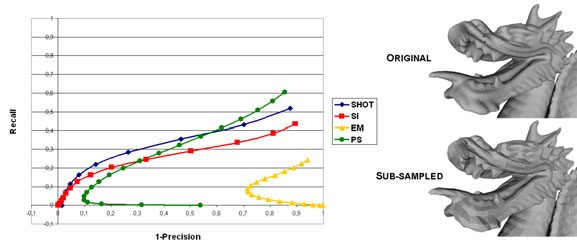
\includegraphics[width=\textwidth]{topics/vergleich/subSampled.png}
}

\frame{
	\frametitle{Ergebnis: Versuch 3}
	\centering
	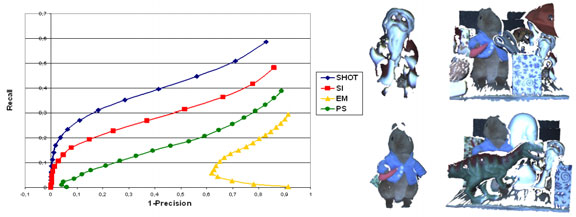
\includegraphics[width=\textwidth]{topics/vergleich/v3.png}
}